\documentclass[12pt,reqno]{article}
\usepackage{amsthm, amsmath, amsfonts, amssymb, amscd, mathtools, youngtab, euscript, mathrsfs, verbatim, enumerate, multicol, multirow, bbding, color, babel, esint, geometry, tikz, tikz-cd, tikz-3dplot, array, enumitem, hyperref, thm-restate, thmtools, datetime, graphicx, tensor, braket, slashed, standalone, pgfplots, ytableau, subfigure, wrapfig, dsfont, setspace, wasysym, pifont, float, rotating, adjustbox, pict2e,array}
\usepackage{amsmath}
\usepackage[utf8]{inputenc}
\usetikzlibrary{arrows, positioning, decorations.pathmorphing, decorations.pathreplacing, decorations.markings, matrix, patterns}
\tikzset{big arrow/.style={
    decoration={markings,mark=at position 1 with {\arrow[scale=1.5,#1]{>}}},
    postaction={decorate},
    shorten >=0.4pt},
  big arrow/.default=black}

\begin{document}

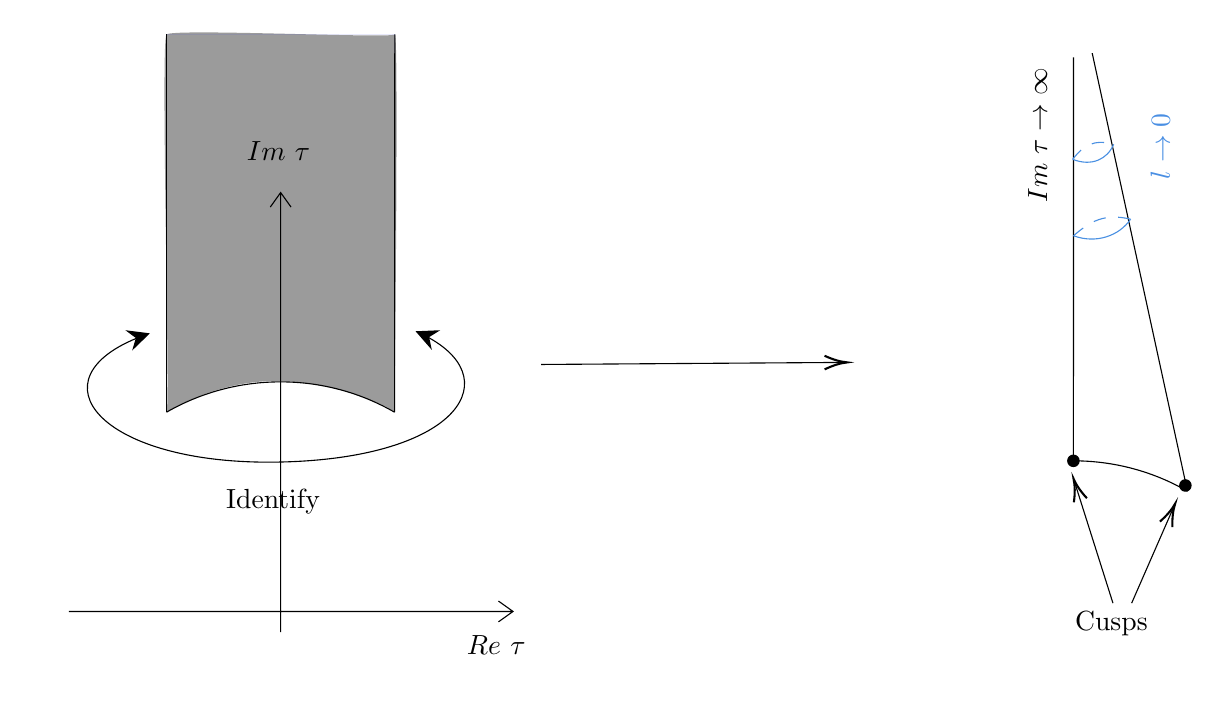
\begin{tikzpicture}[x=0.75pt,y=0.75pt,yscale=-1,xscale=1]
\draw  [draw opacity=0][fill={rgb, 255:red, 155; green, 155; blue, 155 }  ,fill opacity=1 ] (182.5,11) .. controls (184.5,9) and (182.29,194) .. (182.39,193) .. controls (182.5,192) and (158.5,179) .. (127.5,178) .. controls (96.5,177) and (70.5,194) .. (72.5,193) .. controls (74.5,192) and (69.5,14) .. (72.5,11) .. controls (75.5,8) and (180.5,13) .. (182.5,11) -- cycle ;
\draw [fill={rgb, 255:red, 74; green, 80; blue, 226 }  ,fill opacity=1 ]   (72.5,11) -- (72.5,193) ;
\draw [fill={rgb, 255:red, 74; green, 80; blue, 226 }  ,fill opacity=1 ]   (182.5,11) -- (182.39,193) ;
\draw [draw opacity=0][fill={rgb, 255:red, 74; green, 80; blue, 226 }  ,fill opacity=1 ]   (72.5,11) -- (182.5,11) ;
\draw  [draw opacity=0] (72.5,193) .. controls (88.67,183.7) and (107.44,178.38) .. (127.45,178.38) .. controls (147.46,178.38) and (166.22,183.7) .. (182.39,193) -- (127.45,288.17) -- cycle ; \draw   (72.5,193) .. controls (88.67,183.7) and (107.44,178.38) .. (127.45,178.38) .. controls (147.46,178.38) and (166.22,183.7) .. (182.39,193) ;
\draw  (25.45,289) -- (239.45,289)(127.5,87.17) -- (127.5,299) (232.45,284) -- (239.45,289) -- (232.45,294) (122.5,94.17) -- (127.5,87.17) -- (132.5,94.17)  ;
\draw    (61.01,156.23) .. controls (5.88,176.74) and (40.28,218.96) .. (127.5,217) .. controls (214.72,215.04) and (238.07,175.62) .. (195.21,155.22) ;
\draw [shift={(192.5,154)}, rotate = 23.27] [fill={rgb, 255:red, 0; green, 0; blue, 0 }  ][line width=0.08]  [draw opacity=0] (10.72,-5.15) -- (0,0) -- (10.72,5.15) -- (7.12,0) -- cycle    ;
\draw [shift={(64.5,155)}, rotate = 161.57] [fill={rgb, 255:red, 0; green, 0; blue, 0 }  ][line width=0.08]  [draw opacity=0] (10.72,-5.15) -- (0,0) -- (10.72,5.15) -- (7.12,0) -- cycle    ;
\draw    (253,170) -- (398.5,169.01) ;
\draw [shift={(400.5,169)}, rotate = 179.61] [color={rgb, 255:red, 0; green, 0; blue, 0 }  ][line width=0.75]    (10.93,-3.29) .. controls (6.95,-1.4) and (3.31,-0.3) .. (0,0) .. controls (3.31,0.3) and (6.95,1.4) .. (10.93,3.29)   ;
\draw  [draw opacity=0] (509.45,216.42) .. controls (509.45,216.42) and (509.45,216.42) .. (509.45,216.42) .. controls (509.45,216.42) and (509.45,216.42) .. (509.45,216.42) .. controls (529.46,216.42) and (548.22,221.74) .. (564.39,231.04) -- (509.45,326.21) -- cycle ; \draw   (509.45,216.42) .. controls (509.45,216.42) and (509.45,216.42) .. (509.45,216.42) .. controls (509.45,216.42) and (509.45,216.42) .. (509.45,216.42) .. controls (529.46,216.42) and (548.22,221.74) .. (564.39,231.04) ;  
\draw    (509.5,22) -- (509.45,216.42) ;
\draw    (518.5,20) -- (564.39,231.04) ;
\draw [color={rgb, 255:red, 74; green, 144; blue, 226 }  ,draw opacity=1 ]   (509.5,108) .. controls (520.5,112) and (531.5,108) .. (537,100) ;
\draw [color={rgb, 255:red, 74; green, 144; blue, 226 }  ,draw opacity=1 ] [dash pattern={on 4.5pt off 4.5pt}]  (509.5,108) .. controls (517.5,101) and (524.5,97) .. (537,100) ;
\draw [color={rgb, 255:red, 74; green, 144; blue, 226 }  ,draw opacity=1 ]   (509.09,71.15) .. controls (518.13,74.77) and (525.89,71.15) .. (528.82,63.91) ;
\draw [color={rgb, 255:red, 74; green, 144; blue, 226 }  ,draw opacity=1 ] [dash pattern={on 4.5pt off 4.5pt}]  (509.09,71.15) .. controls (514.09,64.82) and (518.79,61.2) .. (528.82,63.91) ;
\draw  [fill={rgb, 255:red, 0; green, 0; blue, 0 }  ,fill opacity=1 ] (506.7,216.42) .. controls (506.7,214.9) and (507.93,213.67) .. (509.45,213.67) .. controls (510.97,213.67) and (512.2,214.9) .. (512.2,216.42) .. controls (512.2,217.94) and (510.97,219.17) .. (509.45,219.17) .. controls (507.93,219.17) and (506.7,217.94) .. (506.7,216.42) -- cycle ;
\draw  [fill={rgb, 255:red, 0; green, 0; blue, 0 }  ,fill opacity=1 ] (560.64,228.29) .. controls (560.64,226.77) and (561.87,225.54) .. (563.39,225.54) .. controls (564.91,225.54) and (566.14,226.77) .. (566.14,228.29) .. controls (566.14,229.81) and (564.91,231.04) .. (563.39,231.04) .. controls (561.87,231.04) and (560.64,229.81) .. (560.64,228.29) -- cycle ;
\draw    (528.5,285) -- (510.1,226.91) ;
\draw [shift={(509.5,225)}, rotate = 72.43] [color={rgb, 255:red, 0; green, 0; blue, 0 }  ][line width=0.75]    (10.93,-3.29) .. controls (6.95,-1.4) and (3.31,-0.3) .. (0,0) .. controls (3.31,0.3) and (6.95,1.4) .. (10.93,3.29)   ;
\draw    (537.5,285) -- (557.7,238.83) ;
\draw [shift={(558.5,237)}, rotate = 113.63] [color={rgb, 255:red, 0; green, 0; blue, 0 }  ][line width=0.75]    (10.93,-3.29) .. controls (6.95,-1.4) and (3.31,-0.3) .. (0,0) .. controls (3.31,0.3) and (6.95,1.4) .. (10.93,3.29)   ;
% Text Node
\draw (110,61.4) node [anchor=north west][inner sep=0.75pt]    {$Im\ \tau $};
% Text Node
\draw (216,299.4) node [anchor=north west][inner sep=0.75pt]    {$Re\ \tau $};
% Text Node
\draw (100,229) node [anchor=north west][inner sep=0.75pt]   [align=left] {Identify};
% Text Node
\draw (486.4,93) node [anchor=north west][inner sep=0.75pt]  [rotate=-270]  {$Im\ \tau \rightarrow \infty $};
% Text Node
\draw (509,288) node [anchor=north west][inner sep=0.75pt]   [align=left] {Cusps};
% Text Node
\draw (545.4,82) node [anchor=north west][inner sep=0.75pt]  [rotate=-270]  {$\textcolor[rgb]{0.29,0.56,0.89}{l\rightarrow 0}$};
\end{tikzpicture}

\end{document}